\section{Experiments}

\subsection{Direct current measurements}

For direct measurements the meter was connected to the circuit in series (Figure~\ref{fig:direct_schematic}). Measurements were taken for varying circuit resistances.

\begin{figure}[H]
	\centering
	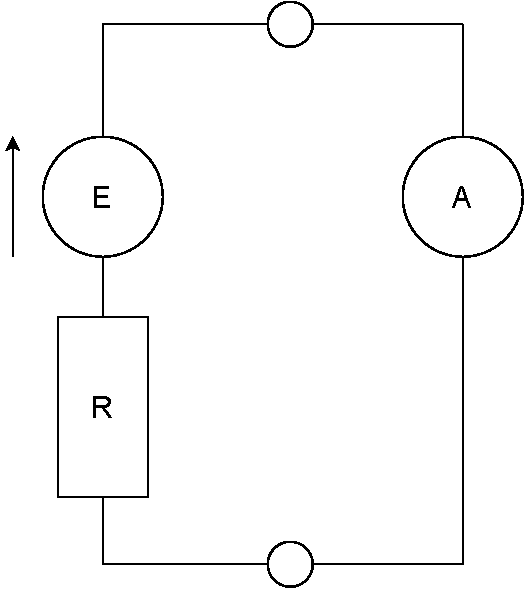
\includegraphics[width=6cm]{schematics/direct.pdf}
	\caption{Direct current measurements schematic}
	\label{fig:direct_schematic}
\end{figure}

\subsubsection{Analog measurements}

The ammeter which we used for analog measurements had a 0.5 accuracy class and a $\frac{23}{I_R  [\unit{\milli\ampere}]} + 0.004 [\unit{\ohm}]$ internal resistance (for: $I_R$ -- range).

The measurements along with the results are split into Tables~\ref{tab:direct_analog_1} and~\ref{tab:direct_analog_2}; Tab.~\ref{tab:direct_analog_1} contains the measurement results with only the limiting error applied, whereas Tab.~\ref{tab:direct_analog_2} shows the final results which include the systematic error.

\begin{table}[H]
	\centering
	\begin{tabular}{ c | c | c | c | c | c | c | c }
		$R_C [\unit{\ohm}]$& $\alpha$ & $\alpha_{max}$ & $I_r [\unit{\milli\ampere}]$ & $I [\unit{\milli\ampere}]$ & $\Delta I [\unit{\milli\ampere}]$ & $\delta I [\unit{\percent}]$ & $I \pm \Delta I [\unit{\milli\ampere}]$\\
		\hline
		10  & 66 & 75 & 150.0 & 132.00 & 0.7500 & 0.56819 & $132.0 \pm 0.8$ \\
		30  & 45 & 75 & 75.0 & 45.00 & 0.3750 & 0.83334 & $45.0 \pm 0.4$ \\
		100  & 67 & 75 & 15.0 & 13.40 & 0.0750 & 0.55971 &  $13.40\pm 0.08$\\
		300  & 45.5 & 75 & 7.5 & 4.55 & 0.0375 & 0.82418 & $4.55 \pm 0.04$\\
		1k  & 34 & 75 & 3.0 & 1.36 & 0.0150 & 1.10295 & $1.360\pm 0.016$\\
		3k  & 12 & 75 & 3.0 & 0.48 & 0.0150 & 3.12501 & $0.480\pm 0.016$\\
		10k  & 5 & 75 & 3.0 & 0.20 & 0.0150 & 7.50001 & $0.200\pm 0.016$\\
	\end{tabular}
	\caption{Current measurements for $E\sim\SI{1.3}{\volt}$ (for: $R_C$ -- circuit resistance, $\alpha$ -- actual needle swing, $\alpha_{max}$ -- maximal swing, $I_r$ -- range, $I$ -- measured current, $\Delta I$ --absolute error, $\delta I$ -- relative error)}
	\label{tab:direct_analog_1}
\end{table}

\begin{table}[H]
	\centering
	\begin{tabular}{c | c | c | c | c | c | c}
		$R_A [\unit{\ohm}]$ & $\Delta_m I [\unit{\milli\ampere}]$ & $\delta_m I$ & $c [\unit{\milli\ampere}]$ & $I_C [\unit{\milli\ampere}]$ & $I_{exp} [\unit{\milli\ampere}]$ & $I_C \pm \Delta I [\unit{\milli\ampere}]$\\
		\hline
		0.15734 & -2.07681 & -0.01550 & 2.07681 & 134.07681 &130.00 & $134.1\pm 0.8$\\
		0.31067 & -0.46601 & -0.01025 & 0.46601 & 45.46601 & 43.33 & $45.5\pm 0.4$\\
		1.53734 & -0.20601 & -0.01515 & 0.20601 & 13.60601  & 13.00 & $13.61\pm 0.08$\\
		3.07067 & -0.04658 & -0.01014 & 0.04658 & 4.59658 & 4.33 & $4.60\pm 0.04$\\
		7.67067 & -0.01044 & -0.00762 & 0.01044 & 1.37044 & 1.30 & $1.370\pm 0.016$\\
		7.67067 & -0.00123 & -0.00256 & 0.00123 & 0.48123 & 0.43 & $0.481\pm 0.016$\\
		7.67067 & -0.00016 & -0.00077 & 0.00016 & 0.20016 & 0.13& $0.200\pm 0.016$\\
	\end{tabular}
	\caption{Current measurements for $E\sim\SI{1.3}{\volt}$ (for: $R_A$ -- internal ammeter resistance, $\Delta_m I$ -- systematic error, $\delta_m I$ -- relative error, $c$ -- correction factor, $I_C$ -- calculated current,  $I_{exp}$ -- expected current)}
	\label{tab:direct_analog_2}
\end{table}

Example calculations for $R_C = \SI{300}{\ohm}$ are shown in the equations below.

\begin{equation}
	I = \frac{\alpha\cdot I_r}{\alpha_{max}} = \frac{45.5\cdot \SI{7.5}{\milli\ampere}}{75} = \SI{4.55}{\milli\ampere}
\end{equation}

\begin{equation}
	\Delta I = \frac{I_r\cdot cl}{100\unit{\percent}} = \frac{\SI{7.5}{\milli\ampere}\cdot 0.5\unit{\percent}}{100\unit{\percent}} = \SI{0.0375}{\milli\ampere}
\end{equation}

\begin{equation}
	\delta I = \frac{\Delta I}{I}\cdot 100\unit{\percent} = \frac{\SI{0.0375}{\milli\ampere}}{\SI{4.55}{\milli\ampere}}\cdot 100\unit{\percent} \approx 0.82418\unit{\percent}
\end{equation}

\begin{equation}
	R_A = \frac{23}{I_R  [\unit{\milli\ampere}]} + 0.004 [\unit{\ohm}] = \frac{23}{\SI{7.5}{\milli\ampere}} + \SI{0.004}{\ohm} \approx \SI{3.07067}{\ohm}
\end{equation}

\begin{equation}
	\Delta_m I = -I_A \cdot\frac{R_A}{R_C} = -\SI{4.55}{\milli\ampere}\cdot\frac{\SI{3.07067}{\ohm}}{\SI{300}{\ohm}} \approx -\SI{0.04658}{\milli\ampere}
\end{equation}

\begin{equation}
	\delta_m I = -\frac{R_A}{R_A + R_C} = -\frac{\SI{3.07067}{\ohm}}{\SI{3.07067}{\ohm} + \SI{300}{\ohm}} \approx -0.01014
\end{equation}

\begin{equation}
	c = -\Delta_m I = -(-\SI{0.04658}{\milli\ampere}) = \SI{0.04658}{\milli\ampere}
\end{equation}

\begin{equation}
	I_C = I + c = \SI{4.55}{\milli\ampere} +\SI{0.04658}{\milli\ampere} = \SI{4.59658}{\milli\ampere}
\end{equation}

\begin{equation}
	I_{exp} = \frac{V}{R_C} = \frac{\SI{1.3}{\volt}}{\SI{300}{\ohm}} \approx \SI{0.00433}{\ampere} = \SI{4.33}{\milli\ampere}
\end{equation}

\subsubsection{Digital measurements}

Digital measurements were made using a multimeter. Its internal resistance, accuracy, and burden voltage for each range are available in the device manual; for our calculations we chose the least precise accuracy value that is guaranteed to work for one year after device calibration.

The measurements along with the results are split into Tables~\ref{tab:direct_digital_1} and~\ref{tab:direct_digital_2}; Tab.~\ref{tab:direct_digital_1} contains the measurement results with only the limiting error applied, whereas Tab.~\ref{tab:direct_digital_2} shows the final results which include the systematic error.

\begin{table}[H]
	\centering
	\begin{tabular}{ c | c | c | c | c | c | c }
		$R_C [\unit{\ohm}]$& Accuracy & $I_r [\unit{\milli\ampere}]$ & $I [\unit{\milli\ampere}]$ & $\Delta I [\unit{\milli\ampere}]$ & $\delta I [\unit{\percent}]$ & $I \pm \Delta I [\unit{\milli\ampere}]$\\
		\hline
		10	& $0.050 + 0.005$	& 100	& 86.4317	 & 0.04822	& 0.05579	& $86.43 \pm 0.05$\\
		30 & $	0.050+0.005$	& 100	& 37.9869	& 0.02400	& 0.06316	&$ 37.987 \pm 0.024$\\
		100	& $0.050+0.005$	& 100	& 12.8199	& 0.01141&	0.08900	 &$12.820 \pm 0.012$\\
		300	&$0.050+0.020$&	10&	4.43229	&0.00422&	0.09512&	$4.432 \pm 0.005$\\
		1000&	$0.050+0.020$	&10	&1.34645&	0.00268	&0.19854&	$1.346 \pm 0.003$\\
		3000&	$0.050+0.020$&	10	&0.45049&	0.00223	&0.49396&	$0.4505 \pm0.0023$\\
		10000	&$0.050+0.020$&	10&	0.13522	&0.00207&	1.52907&	$0.1352 \pm 0.0021$\\
	\end{tabular}
	\caption{Current measurements for $E\sim\SI{1.3}{\volt}$ (for: $R_C$ -- circuit resistance, Accuracy: $\pm$ (a$\unit{\percent}$ of reading + b$\unit{\percent}$ of range), $I_r$ -- range, $I$ -- measured current, $\Delta I$ --absolute error, $\delta I$ -- relative error)}
	\label{tab:direct_digital_1}
\end{table}

\begin{table}[H]
	\centering
	\begin{tabular}{c | c | c | c | c | c | c}
		$R_A [\unit{\ohm}]$ & $\Delta_m I [\unit{\milli\ampere}]$ & $\delta_m I$ & $c [\unit{\milli\ampere}]$ & $I_C [\unit{\milli\ampere}]$ & $I_{exp} [\unit{\milli\ampere}]$ & $I_C \pm \Delta I [\unit{\milli\ampere}]$\\
		\hline
		6	& -51.85903&	-0.37501&	51.85903&	138.29073&	130.00& $138.29\pm 0.05$\\
		6&	-7.59739&	-0.16667&	7.59739&	45.58429&	43.33&$45.584\pm 0.024$\\
		6	&-0.76920	&-0.05661&	0.76920&	13.58910&	13.00& $13.589\pm 0.012$\\
		10	&-0.14775&	-0.03226&	0.14775&	4.58004&	4.33& $4.580\pm 0.005$\\
		10&	-0.01347&	-0.00991&	0.01347&	1.35992&	1.30& $1.360\pm 0.003$\\
		10&	-0.00151&	-0.00333&	0.00151&	0.45200&	0.43&$0.4520\pm 0.0023$\\
		10&	-0.00014&	-0.00010&	0.00014&	0.13536&	0.13& $0.1354\pm 0.0021$\\
	\end{tabular}
	\caption{Current measurements for $E\sim\SI{1.3}{\volt}$ (for: $R_A$ -- internal multimeter resistance, $\Delta_m I$ -- systematic error, $\delta_m I$ -- relative error, $c$ -- correction factor, $I_C$ -- calculated current,  $I_{exp}$ -- expected current)}
	\label{tab:direct_digital_2}
\end{table}

Example calculations for $R_C = \SI{300}{\ohm}$ are shown in the equations below.

\begin{equation}
	\begin{split}
		\Delta I &= \frac{a}{100\unit{\percent}}\cdot I + 	\frac{b}{100\unit{\percent}}\cdot I_r = \frac{0.050\unit{\percent}}{100\unit{\percent}}\cdot\SI{4.43229}{\milli\ampere} + \frac{0.020\unit{\percent}}{100\unit{\percent}}\cdot\SI{10}{\milli\ampere} =\\
		&= \SI{0.002216145}{\milli\ampere} + \SI{0,002}{\milli\ampere} = \SI{0.004216145}{\milli\ampere}\approx\SI{0.00422}{\milli\ampere}
	\end{split}
\end{equation}

\begin{equation}
	\delta I = \frac{\Delta I}{I}\cdot 100\unit{\percent} = \frac{\SI{0.00422}{\milli\ampere}}{\SI{4.43229}{\milli\ampere}}\cdot 100\unit{\percent} \approx 0.09521\unit{\percent}
\end{equation}

\begin{equation}
	R_A = \frac{\text{burden voltage}}{I_R  [\unit{\milli\ampere}]} = \frac{\SI{0.1}{\volt}}{\SI{10}{\milli\ampere}}=\frac{\SI{0.1}{\volt}}{\SI{0.01}{\ampere}}=\SI{10}{\ohm}
\end{equation}

\begin{equation}
	\Delta_m I = -I_A \cdot\frac{R_A}{R_C} = -\SI{4.43229}{\milli\ampere}\cdot\frac{\SI{10}{\ohm}}{\SI{300}{\ohm}} \approx -\SI{0.14775}{\milli\ampere}
\end{equation}

\begin{equation}
	\delta_m I = -\frac{R_A}{R_A + R_C} = -\frac{\SI{10}{\ohm}}{\SI{10}{\ohm} + \SI{300}{\ohm}} \approx -0.032256
\end{equation}

\begin{equation}
	c = -\Delta_m I = -(-\SI{0.14775}{\milli\ampere}) =  \SI{0.14775}{\milli\ampere}
\end{equation}

\begin{equation}
	I_C = I + c =\SI{4.43229}{\milli\ampere} +\SI{0.14775}{\milli\ampere} = \SI{4.58004}{\milli\ampere}
\end{equation}

\begin{equation}
	I_{exp} = \frac{V}{R_C} = \frac{\SI{1.3}{\volt}}{\SI{300}{\ohm}} \approx \SI{0.00433}{\ampere} = \SI{4.33}{\milli\ampere}
\end{equation}


\subsection{Indirect current measurement}

To take indirect current measurements, we added an extra resistance standard to the circuit (Figure~\ref{fig:indirect_schematic}) and measured the voltage drop across it Voltage was measured with a digital multimeter, connected to the circuit in parallel. Measurements were taken for varying circuit and resistance standard values and current was calculated using Ohm's law.

The measurements along with the results are split into Tables~\ref{tab:indirect_digital_1},~\ref{tab:indirect_digital_2} and~\ref{tab:indirect_digital_3}; Tab.~\ref{tab:indirect_digital_1} and~\ref{tab:indirect_digital_2} contain the measurement results with only the limiting error applied, whereas Tab.~\ref{tab:indirect_digital_3} shows the final results which include the systematic error.

\begin{figure}[H]
	\centering
	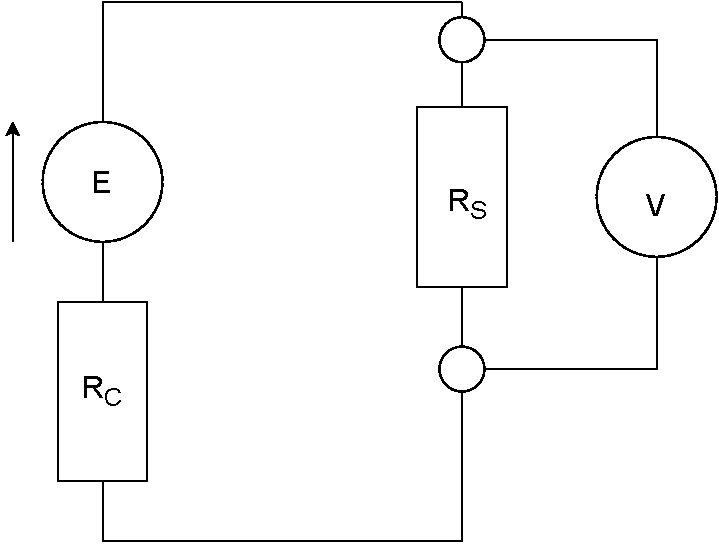
\includegraphics[width=8cm]{schematics/indirect.pdf}
	\caption{Indirect current measurements schematic}
	\label{fig:indirect_schematic}
\end{figure}

\begin{table}[H]
	\centering
	\begin{tabular}{ c | c | c | c | c | c  }
		$R_C [\unit{\ohm}]$& Accuracy & $V_r [\unit{\volt}]$ & $V [\unit{\volt}]$ & $\Delta V [\unit{\volt}]$ & $\delta V [\unit{\percent}]$ \\
		\hline
			10	& 0.0035+0.0005	& 10	& 1.22609&	0.00009294 &	0.00757801\\
			100	& 0.0040+0.0007	&1&	0.675053	& 0.00003401&0.00503696\\
			1000 &	0.0040+0.0007	&1&	0.122755	&0.00001192&	0.00971040\\
			10000	& 0.0050+0.0035	&0.1&	0.013375&	0.00000417 &	0.03116744\\
			10	&0.0040+0.0007	&1&	0.658095&	0.00003333 &	0.00506368\\
			100	&0.0040+0.0007	&1	&0.122238	&0.00001189&	0.00972653\\
			1000	&0.0050+0.0035&	0.1&	0.013369&	0.00000417&	0.03118016\\
			10000&	0.0050+0.0035	&0.1&	0.001348&	0.00000357&	0.26458615\\
			10	& 0.0035+0.0005	&10	&1.33556 &	0.00009675&	0.00724375\\
			100	&0.0035+0.0005	&10&	1.22532&	0.00009289&	0.00758057\\
			1000	&0.0040+0.0007	&1&	0.673799	&0.00003396&	0.00503889\\
			10000	&0.0040+0.0007	&1&	0.122527	&0.00001191&	0.00971303\\
	\end{tabular}
	\caption{Current measurements for $E\sim\SI{1.3}{\volt}$ (for: $R_C$ -- circuit resistance, Accuracy: $\pm$ (a$\unit{\percent}$ of reading + b$\unit{\percent}$ of range), $V_r$ -- range, $V$ -- measured voltage, $\Delta V$ --absolute error, $\delta V$ -- relative error)}
	\label{tab:indirect_digital_1}
\end{table}

\begin{table}[H]
	\centering
	\begin{tabular}{ c | c | c | c | c | c  }
		$R_S [\unit{\ohm}]$& cl & $I [\unit{\milli\ampere}]$ & $\Delta I [\unit{\milli\ampere}]$ & $\delta I [\unit{\percent}]$ & $I \pm \Delta I [\unit{\milli\ampere}]$\\
		\hline
		100	& 0.01 & 12.26090	& 0.00216	& 0.017588 & $12.2609\pm 0.0022$\\
		100	&0.01	&6.75053	&0.00102	&0.015037&$6.7505\pm 0.0011$\\
		100	&0.01	&1.22755&	0.00025	&0.019710&$1.2276 \pm 0.0003$\\
		100	&0.01&	0.13375	&0.00006&	0.041167&$0.13375\pm 0.00006$\\
		10	&0.01	&65.80950	&0.00992&	0.015064&$65.81\pm 0.01$\\
		10	&0.01	&12.22380	&0.00242	&0.019727&$12.2238\pm 0.0025$\\
		10	&0.01	&1.33689	&0.00056	&0.041180&$1.3369 \pm 0.0006$\\
		10	&0.01	&0.13483	&0.00038	&0.274586&$0.1348\pm 0.0004$\\
		1000&	0.01&	1.33556	&0.00024&	0.017244&$1.33556\pm 0.00024$\\
		1000&	0.01&	1.22532	&0.00022	&0.017581&$1.22532\pm 0.00022$\\
		1000&	0.01&	0.67380	&0.00011	&0.015039& $0.67380\pm 0.00012$\\
		1000&	0.01&	0.12253	&0.00003	&0.019713&$0.12253\pm 0.00003$\\
	\end{tabular}
	\caption{Current measurements for $E\sim\SI{1.3}{\volt}$ (for: $R_C$ -- resistance standard, cl -- resistance standard class, $I$ -- measured current, $\Delta I$ --  absolute error, $\delta I$ --relative error)}
	\label{tab:indirect_digital_2}
\end{table}

\begin{table}[H]
	\centering
	\begin{tabular}{ c | c | c | c | c  }
	$\Delta_m I [\unit{\milli\ampere}]$ & $\delta_m I $ & $c [\unit{\milli\ampere}]$ & $ I_C [\unit{\milli\ampere}]$ & $I_C \pm \Delta I [\unit{\milli\ampere}]$\\
		\hline
		-122.60901	&-0.90909	&122.60901	&134.86990&$134.8610\pm 0.0022$\\
		-6.75054	&-0.50000	&6.75054	&13.50106&$13.5011\pm 0.0011$\\
		-0.12276	&-0.09091	&0.12276	&1.35031&$1.3503\pm 0.0003$\\
		-0.00134	&-0.00990	&0.00134	&0.13509&$0.13510\pm 0.00006$\\
		-65.80951&	-0.50000	&65.80951	&131.61900&$131.62\pm 0.01$\\
		-1.22239	&-0.09091	&1.22239	&13.44618&$13.4462\pm 0.0025$\\
		-0.01337	&-0.00990	&0.01337	&1.35026&$1.3503\pm 0.0006$\\
		-0.00014	&-0.00091	&0.00014	&0.13496&$0.1350\pm 0.0004$\\
		-133.55601	&-0.99001	&133.55601	&134.89156&$134.8916\pm 0.0024$\\
		-12.25321	&-0.90909	&12.25321&	13.47852&$13.47852\pm 0.00022$\\
		-0.67380	&-0.50000	&0.67380&	1.34769&$1.34770\pm 0.00012$\\
		-0.01226	&-0.09091	&0.01226&	0.13478&$0.13478\pm 0.00003$\\
	\end{tabular}
	\caption{Current measurements for $E\sim\SI{1.3}{\volt}$ (for: $\Delta_m I$ --  systematic error, $\delta_m I$ --  relative error, $c$ -- correction factor, $ I_C$ --  calculated current)}
	\label{tab:indirect_digital_3}
\end{table}

Example calculations for $R_C = \SI{1000}{\ohm}$ and $R_S = \SI{100}{\ohm}$ are shown in the equations below.

\begin{equation}
	\begin{split}
		\Delta V &= \frac{a}{100\unit{\percent}}\cdot V + 	\frac{b}{100\unit{\percent}}\cdot V_r = \frac{0.0040\unit{\percent}}{100\unit{\percent}}\cdot\SI{0.122755}{\volt} + \frac{0.0007\unit{\percent}}{100\unit{\percent}}\cdot\SI{1}{\volt} =\\
		&= \SI{0.0000049102}{\volt} + \SI{0.000007}{\volt} = \SI{0.0000119102}{\volt}\approx\SI{0.00001192}{\volt}
	\end{split}
\end{equation}

\begin{equation}
	\delta V = \frac{\Delta V}{V}\cdot 100\unit{\percent} = \frac{\SI{0.00001192}{\volt}}{\SI{0.122755}{\volt}}\cdot 100\unit{\percent} \approx 0.00971040 \unit{\percent}
\end{equation}

\begin{equation}
	I = \frac{V}{R_S} = \frac{\SI{0.122755}{\volt}}{\SI{100}{\ohm}} = \SI{0.00122755}{\ampere} = \SI{1.22755}{\milli\ampere}
\end{equation}

\begin{equation}
	\delta I = \delta V + \delta R_S = \delta V + cl =  0.00971040\unit{\percent} + 0.01\unit{\percent} \approx 0.01971\unit{\percent}
\end{equation}

\begin{equation}
	\Delta I = \frac{I\cdot\delta I}{100\unit{\percent}} = \frac{ \SI{1.22755}{\milli\ampere}\cdot  0.01971\unit{\percent}}{100\unit{\percent}} = \SI{0.000241950105}{\milli\ampere}\approx\SI{ 0.00025}{\milli\ampere}
\end{equation}

\begin{equation}
	\Delta_m I = -I_A \cdot\frac{R_A}{R_C} = -I_A \cdot\frac{R_S}{R_C} = - \SI{1.22755}{\milli\ampere}\cdot\frac{\SI{100}{\ohm}}{\SI{1000}{\ohm}} \approx -\SI{0.12276}{\milli\ampere}
\end{equation}

\begin{equation}
	\delta_m I = -\frac{R_A}{R_A + R_C} = -\frac{R_S}{R_S + R_C} = -\frac{\SI{100}{\ohm}}{\SI{100}{\ohm} + \SI{1000}{\ohm}} \approx -0.09091
\end{equation}

\begin{equation}
	c = -\Delta_m I = -(-\SI{0.12276}{\milli\ampere}) =  \SI{0.12276}{\milli\ampere}
\end{equation}

\begin{equation}
	I_C = I + c = \SI{1.22755}{\milli\ampere} +\SI{0.12276}{\milli\ampere} \approx \SI{1.35031}{\milli\ampere}
\end{equation}





